\section{Dados Abertos}

Este trabalho se fundamenta na disponibilização de dados governamentais em formato aberto, livre de restrições de direitos autorais ou outros mecanismos de controle. Conforme definido pelo movimento OK Brasil \cite{OKBrasil2024} e pelo Arquivo Nacional do Reino Unido \cite{ArquivoNacional2023}, os "dados abertos" são aqueles disponibilizados livremente para acesso, uso, reutilização e redistribuição por qualquer indivíduo. Para que sejam considerados como tal, é crucial que os dados estejam em formatos abertos e não proprietários, permitindo a sua fácil integração com outros sistemas e ferramentas.

No contexto da pesquisa científica, os dados abertos são essenciais para a aceleração de descobertas e a promoção da colaboração \cite{SayaoSales2014}. Ao tornar dados disponíveis em formato aberto, pesquisadores e cientistas sociais ganham condições concretas para replicar estudos, contestar resultados e explorar perspectivas de análise que dependem do acesso livre a fontes primárias. Sayão e Sales \cite{SayaoSales2014} argumentam que essa abertura não é apenas uma mudança técnica, mas uma transformação nas práticas de comunicação científica, exigindo novas formas de gerenciamento, preservação e compartilhamento de dados ao longo do tempo.

Na gestão pública, os dados abertos são fundamentais para a transparência e a accountability. Ao disponibilizar dados sobre gastos públicos e contratos governamentais, os governos aumentam sua transparência e permitem um controle social mais rigoroso \cite{ZuiderwijkJanssen2014}. No Brasil, a API do Senado Federal configura-se como uma ferramenta essencial para a democracia participativa, oferecendo dados brutos sobre o funcionamento da Instituição. Contudo, a efetividade dessa abertura depende da qualidade com que os dados são entregues aos cidadãos. Conforme argumentado por Vetro et al. \cite{Vetro2016}, a qualidade dos dados deve ser observada em todas as etapas de sua disponibilização, desde a coleta até a apresentação. A Figura \ref{fig:processo_publicacao} ilustra o processo de publicação de dados abertos e os pontos críticos onde a intervenção técnica é necessária para assegurar que o dado bruto se torne informação útil.

\begin{figure}[H]
\centering
\caption{Processo de publicação e estruturação de dados abertos}
\label{fig:processo_publicacao}
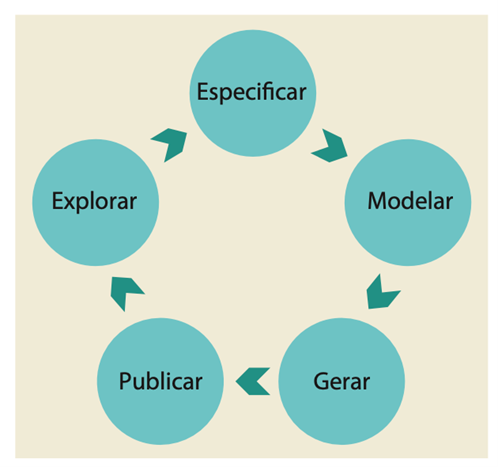
\includegraphics[width=0.6\textwidth]{imagens/publicacao.png}
\fonte{Adaptado de Villazón-Terrazas et al. (2011).}
\end{figure}

\subsection{As 5 Estrelas dos Dados Abertos}

Para maximizar o potencial de reutilização e interoperabilidade dos dados abertos, Tim Berners-Lee propôs um sistema de classificação de 5 estrelas (Figura \ref{fig:5_estrelas}), que gradua o nível de abertura e estruturação dos dados \cite{IsotaniBittencourt2015}. A seguir, são descritas cada uma das etapas:

\begin{itemize}
\item \textbf{1 estrela:} Disponível na web (qualquer formato) com licença aberta. Este é o nível mais básico de abertura de dados.
\item \textbf{2 estrelas:} Disponível como dados estruturados (por exemplo, em formatos CSV ou Excel). Nesse estágio, os dados são organizados em tabelas ou outras estruturas que facilitam a sua manipulação e análise.
\item \textbf{3 estrelas:} Como 2 estrelas, mas em formato não proprietário. Aqui, os dados estão disponíveis em formatos abertos padronizados (como CSV), o que facilita sua integração com diversas ferramentas de visualização e análise.
\item \textbf{4 estrelas:} Como 3 estrelas, mais uso de URIs e padrões W3C (RDF, SPARQL). Neste estágio, os dados são identificáveis na web através de URIs, o que permite a sua ligação com outras fontes de informação. Os dados também podem ser descritos em formato RDF, permitindo a sua integração com recursos semânticos padronizados.
\item \textbf{5 estrelas:} Como 4 estrelas, mais ligação (link) com outros dados para fornecer contexto (\textit{Linked Data}). Neste ponto, os dados não apenas são abertos e interoperáveis, mas também estão conectados a outras fontes de informação relevantes. Isso permite a construção de aplicações que fornecem uma visão holística dos dados.
\end{itemize}

\begin{figure}[H]
\centering
\caption{Diagrama das 5 estrelas de Dados Abertos}
\label{fig:5_estrelas}
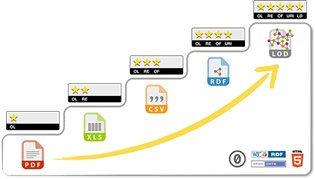
\includegraphics[width=0.8\textwidth]{imagens/estrelas.png}
\fonte{5stardata.info.}
\end{figure}

\section{Processamento de Linguagem Natural (PLN) e Modelos de Linguagem}

O Processamento de Linguagem Natural (PLN) é uma subárea da Inteligência Artificial que se dedica a capacitar os computadores para processar e compreender a linguagem humana \cite{JurafskyMartin2023}. A abordagem clássica do PLN exigia um \textit{pipeline} complexo de pré-processamento manual e intensivo (Figura \ref{fig:pln_classico}), onde o texto era convertido em representações vetoriais numéricas.

\begin{figure}[H]
\centering
\caption{Abordagem Clássica de PLN}
\label{fig:pln_classico}
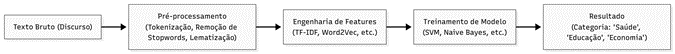
\includegraphics[width=0.8\textwidth]{imagens/abordagem_pln.png}
\fonte{Produção da autora.}
\end{figure}

Com o advento dos Modelos de Linguagem de Larga Escala (LLMs), essa abordagem mudou drasticamente. Como ilustrado na Figura \ref{fig:pln_generativo}, os LLMs são capazes de realizar tarefas complexas, como tradução, resumo e geração de texto, de forma \textit{end-to-end}, sendo instruídos por comandos em linguagem natural (\textit{prompts}).

\begin{figure}[H]
\centering
\caption{Abordagem Generativa com LLMs}
\label{fig:pln_generativo}
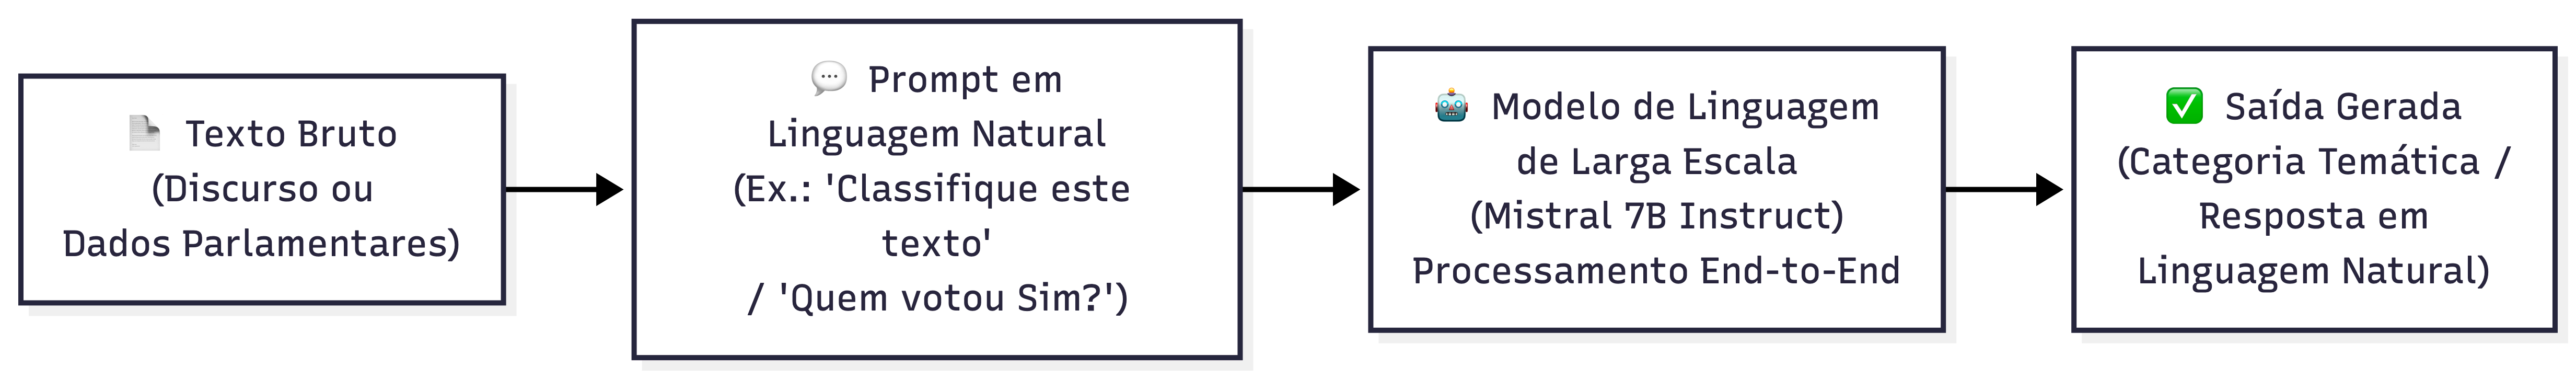
\includegraphics[width=0.8\textwidth]{imagens/abordagem_generativa.png}
\fonte{Produção da autora.}
\end{figure}

Este trabalho adota a abordagem generativa, utilizando o modelo Mistral 7B Instruct \cite{MistralAI2024}, que roda em ambiente local para executar tarefas de classificação temática e resposta a perguntas (\textit{Question Answering}), dispensando a necessidade de treinamento de modelos específicos para cada tarefa e evitando dependência de APIs externas.

\section{Inteligência Artificial Generativa}

Os Modelos de Linguagem de Larga Escala (LLMs) são modelos fundamentados em arquiteturas de redes neurais profundas (\textit{deep learning}), treinados com volumes massivos de dados para compreender e gerar linguagem com alta fluência \cite{RedHat2023}. O fluxo típico de desenvolvimento desses modelos envolve coleta, treinamento e refinamento por \textit{feedback} humano (RLHF), conforme a Figura \ref{fig:fluxo_llm}.

\begin{figure}[H]
\centering
\caption{Fluxo de Treinamento e Refinamento de um LLM}
\label{fig:fluxo_llm}
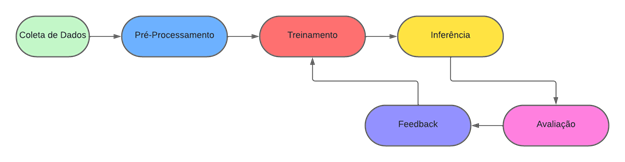
\includegraphics[width=0.8\textwidth]{imagens/llm.png}
\fonte{Produção da autora.}
\end{figure}

No contexto desta pesquisa, a IA Generativa é empregada para classificar discursos parlamentares por tema e gerar respostas em linguagem natural a partir de dados legislativos estruturados \cite{Tamper2022}. Esse uso, porém, não é isento de riscos: alucinações — respostas factualmente incorretas geradas com aparente confiança pelo modelo — e vieses presentes nos dados de treinamento representam ameaças concretas à confiabilidade do sistema \cite{MarquesLaipelt2023}. Em contextos cívicos, onde informação imprecisa pode influenciar a percepção pública sobre representantes políticos, esses riscos não podem ser tratados apenas como limitações técnicas; eles exigem mecanismos explícitos de verificação e rastreabilidade, que constituem, precisamente, um dos focos desta dissertação.

\subsection{Recuperação Aumentada por Geração}

Além da geração textual, este trabalho adota uma estratégia de Recuperação Aumentada por Geração (\textit{Retrieval-Augmented Generation} -- RAG). Em linhas gerais, RAG combina uma etapa de recuperação de informações relevantes em uma base de dados ou coleção documental com uma etapa de geração de resposta por modelo de linguagem \cite{Lewis2020}. Essa abordagem é adequada para domínios em que a resposta deve permanecer ancorada em fontes verificáveis, pois o modelo não responde apenas com base em seus parâmetros internos: ele recebe, no \textit{prompt}, um contexto recuperado previamente.

No AgentAI, a etapa de recuperação não emprega indexação vetorial densa com modelos de \textit{embedding} e operações de similaridade semântica, mas sim \textbf{busca estruturada} sobre a base local --- filtrando registros por parlamentar, período, tema ou palavras presentes no texto --- e fornece esse contexto diretamente ao Mistral 7B Instruct para a geração da resposta. Por rigor terminológico, esta dissertação refere-se a tal estratégia como \textit{recuperação estruturada com geração aumentada} (uma abordagem inspirada em RAG), reservando o termo RAG, em sentido estrito \cite{Lewis2020}, para arquiteturas que realizam recuperação por similaridade semântica densa. Essa escolha implica um \textit{trade-off} explícito: perde-se a capacidade de recuperar documentos por paráfrase ou sinônimo (limitação que será documentada na avaliação), mas ganha-se rastreabilidade direta --- cada resposta pode ser associada aos registros exatos que a fundamentaram. Para o objetivo desta dissertação, que é justamente investigar a qualidade factual e a rastreabilidade das respostas em contexto legislativo, essa abordagem é metodologicamente coerente.

\subsection{Mistral 7B Instruct vs. Alternativas}
\label{subsec:escolha_modelo}

A escolha do modelo Mistral 7B Instruct justifica-se por múltiplos aspectos técnicos e científicos. Diferentemente de APIs proprietárias como Google Gemini, Mistral 7B oferece:

\begin{itemize}
\item \textbf{Privacidade e Soberania de Dados:} O modelo roda localmente, garantindo que os dados legislativos brasileiros não sejam transmitidos para servidores externos, o que se alinha com princípios de soberania digital.
\item \textbf{Replicabilidade:} Por ser \textit{open-source}, permite que outros pesquisadores reproduzam exatamente o experimento e validem os resultados de forma independente, atendendo aos critérios de rigor científico.
\item \textbf{Custo Operacional:} Elimina dependência de APIs pagas, reduzindo barreiras financeiras para a replicação da pesquisa.
\item \textbf{Performance Adequada:} Apesar de menor em parâmetros que os grandes modelos proprietários, o Mistral 7B Instruct apresenta desempenho competitivo em tarefas de compreensão e geração de linguagem em benchmarks gerais \cite{Jiang2023}; sua adequação específica ao domínio legislativo em português constitui, precisamente, uma das questões investigadas nesta dissertação.
\end{itemize}

Este trade-off entre capacidade absoluta (modelos proprietários maiores) e replicabilidade (modelo local open-source) representa uma escolha metodológica consciente que prioriza a sustentabilidade e transparência da pesquisa.

Reconhece-se que o Mistral 7B Instruct, lançado em 2023, não é o modelo aberto mais recente disponível ao tempo de conclusão desta dissertação. A escolha, contudo, prioriza deliberadamente a \textbf{replicabilidade} sobre a recência: um modelo congelado, amplamente documentado e de pesos abertos permite que o experimento seja reproduzido de forma idêntica por terceiros --- garantia que não se obtém com modelos sujeitos a atualizações frequentes ou a descontinuação. Trata-se, portanto, de uma limitação assumida, e não de uma afirmação de superioridade do modelo. Essa opção é viabilizada pela arquitetura modular do artefato quanto ao componente de linguagem: o LLM é acessado por uma interface de inferência padronizada, de modo que a substituição por um modelo mais recente constitui trabalho futuro de baixo custo de integração, sem alteração dos demais estágios de coleta, recuperação e avaliação.

\section{Design Science Research}

O Design Science Research (DSR) é um paradigma metodológico específico para a pesquisa em Ciência da Computação, que combina rigor científico com a construção prática de artefatos tecnológicos \cite{Peffers2007}. Conforme definido por Peffers et al. \cite{Peffers2007}, DSR diferencia-se da pesquisa puramente teórica porque investiga não apenas se um artefato funciona, mas como e por que ele funciona, gerando conhecimento científico sobre seu design, sua implementação, suas limitações e sua avaliação.

Runeson et al. \cite{Runeson2020} complementam ao argumentar que, em Engenharia de Software e Computação, construir um artefato (seja software, hardware ou framework) em si não constitui automaticamente conhecimento científico. O conhecimento emerge quando se documenta e avalia sistematicamente o processo e os impactos daquele artefato. Conforme Pimentel et al. \cite{Pimentel2020}, a pesquisa em Design Science visa "a construção de artefatos como estratégia para o avanço do conhecimento".

\subsection{Fases da Design Science Research}

O ciclo de DSR, conforme proposto por Peffers et al. \cite{Peffers2007}, compreende seis fases que orientam o desenvolvimento de pesquisa em Computação:

\begin{enumerate}
\item \textbf{Motivação e Identificação do Problema:} Definição clara do problema prático que o artefato propõe-se a resolver, fundamentado em literatura e observação empírica.
\item \textbf{Objetivos da Solução:} Especificação do que a solução deve atingir e justificativa teórica para as escolhas de design.
\item \textbf{Design e Desenvolvimento:} Construção do artefato, documentando decisões técnicas e sua fundamentação.
\item \textbf{Demonstração:} Apresentação do artefato funcionando em cenários reais ou controlados, validando a viabilidade técnica.
\item \textbf{Avaliação:} Avaliação rigorosa da efetividade técnica, qualidade das respostas, rastreabilidade e limitações, comparando contra critérios pré-definidos.
\item \textbf{Reflexão e Aprendizados:} Documentação do conhecimento científico gerado, contribuições à teoria, limitações e trabalhos futuros.
\end{enumerate}

\subsection{DSR no Contexto desta Pesquisa}

Este trabalho adota DSR porque seu objetivo central é a construção e avaliação de um artefato computacional (AgentAI) cuja utilidade e eficácia técnica devem ser validadas. Diferentemente de uma pesquisa exploratória que investiga "o que está acontecendo" em um contexto natural, esta pesquisa propõe e testa uma solução, investigando em que medida ela apoia a estruturação, classificação e consulta de dados parlamentares abertos. Conforme argumentado por Thuan et al. \cite{Thuan2019}, ao formular a questão de pesquisa em DSR, deve-se focar em "Como?" (design e implementação) e "Em que medida?" (efetividade do artefato), não apenas "O quê?"

\section{Interação Humano-Dados e Acessibilidade de Informação}

Um dos desafios fundamentais na democratização de dados é garantir que os cidadãos consigam não apenas acessar informações, mas também compreendê-las e interpretá-las adequadamente. Este problema é abordado pela comunidade de pesquisa em Interação Humano-Dados.

\subsection{Desafios de Visualização de Dados}

Lee et al. \cite{Lee2017}, através do desenvolvimento do VLAT (\textit{Visualization Literacy Assessment Test}), demonstraram que nem todos os usuários conseguem interpretar visualizações gráficas complexas. O estudo evidencia que usuários com pouca exposição a gráficos estatísticos cometem com frequência erros na leitura de eixos, escalas e representações multidimensionais, e que visualizações sofisticadas --- como \textit{heatmaps} e \textit{scatter plots} tridimensionais --- podem confundir mais do que esclarecer para quem não domina a linguagem gráfica. A compreensão visual de dados configura-se, assim, como uma competência que varia significativamente entre indivíduos, e não como um pressuposto universal.

\subsection{Barreiras Cognitivas para Usuários Não-Especialistas}

Hornung et al. \cite{Hornung2015} apontam que usuários sem formação em estatística ou ciência de dados frequentemente enfrentam barreiras cognitivas significativas ao tentar analisar dados complexos. Essas barreiras manifestam-se na falta de familiaridade com conceitos como mediana, distribuição e correlação, na dificuldade de formular hipóteses e validá-las contra os dados e na sobrecarga cognitiva decorrente de lidar simultaneamente com múltiplas dimensões de informação.

Consequentemente, a mera disponibilização de dados e interfaces visuais não garante compreensão ou participação democrática efetiva. Conforme Brito et al. \cite{Brito2024}, em seu trabalho sobre "Literacia de Dados para Todos", a solução requer abordagens múltiplas que reduzam progressivamente barreiras de entrada.

\subsection{Interfaces Conversacionais como Estratégia de Acessibilidade}

Neste contexto, interfaces conversacionais alimentadas por modelos de linguagem generativa representam uma estratégia complementar à visualização tradicional. Ao permitir que os usuários formulem perguntas em linguagem natural (por exemplo: "Como votou o Senador X sobre educação?"), reduz-se a necessidade de expertise técnica ou estatística. A IA Generativa traduz a pergunta em operações sobre os dados, apresentando resultados em linguagem acessível.

A combinação de duas modalidades de interação—Dashboard visual e Chatbot conversacional—permite que diferentes usuários escolham a interface que melhor se adequa ao seu estilo cognitivo e nível de expertise, aumentando a acessibilidade global da solução. A arquitetura da aplicação desenvolvida neste trabalho (Figura \ref{fig:arquitetura_interacao}) combina essas duas abordagens para maximizar a acessibilidade.

\begin{figure}[H]
\centering
\caption{Arquitetura de interação do usuário com os dados parlamentares: Dashboard e Chatbot integrados}
\label{fig:arquitetura_interacao}
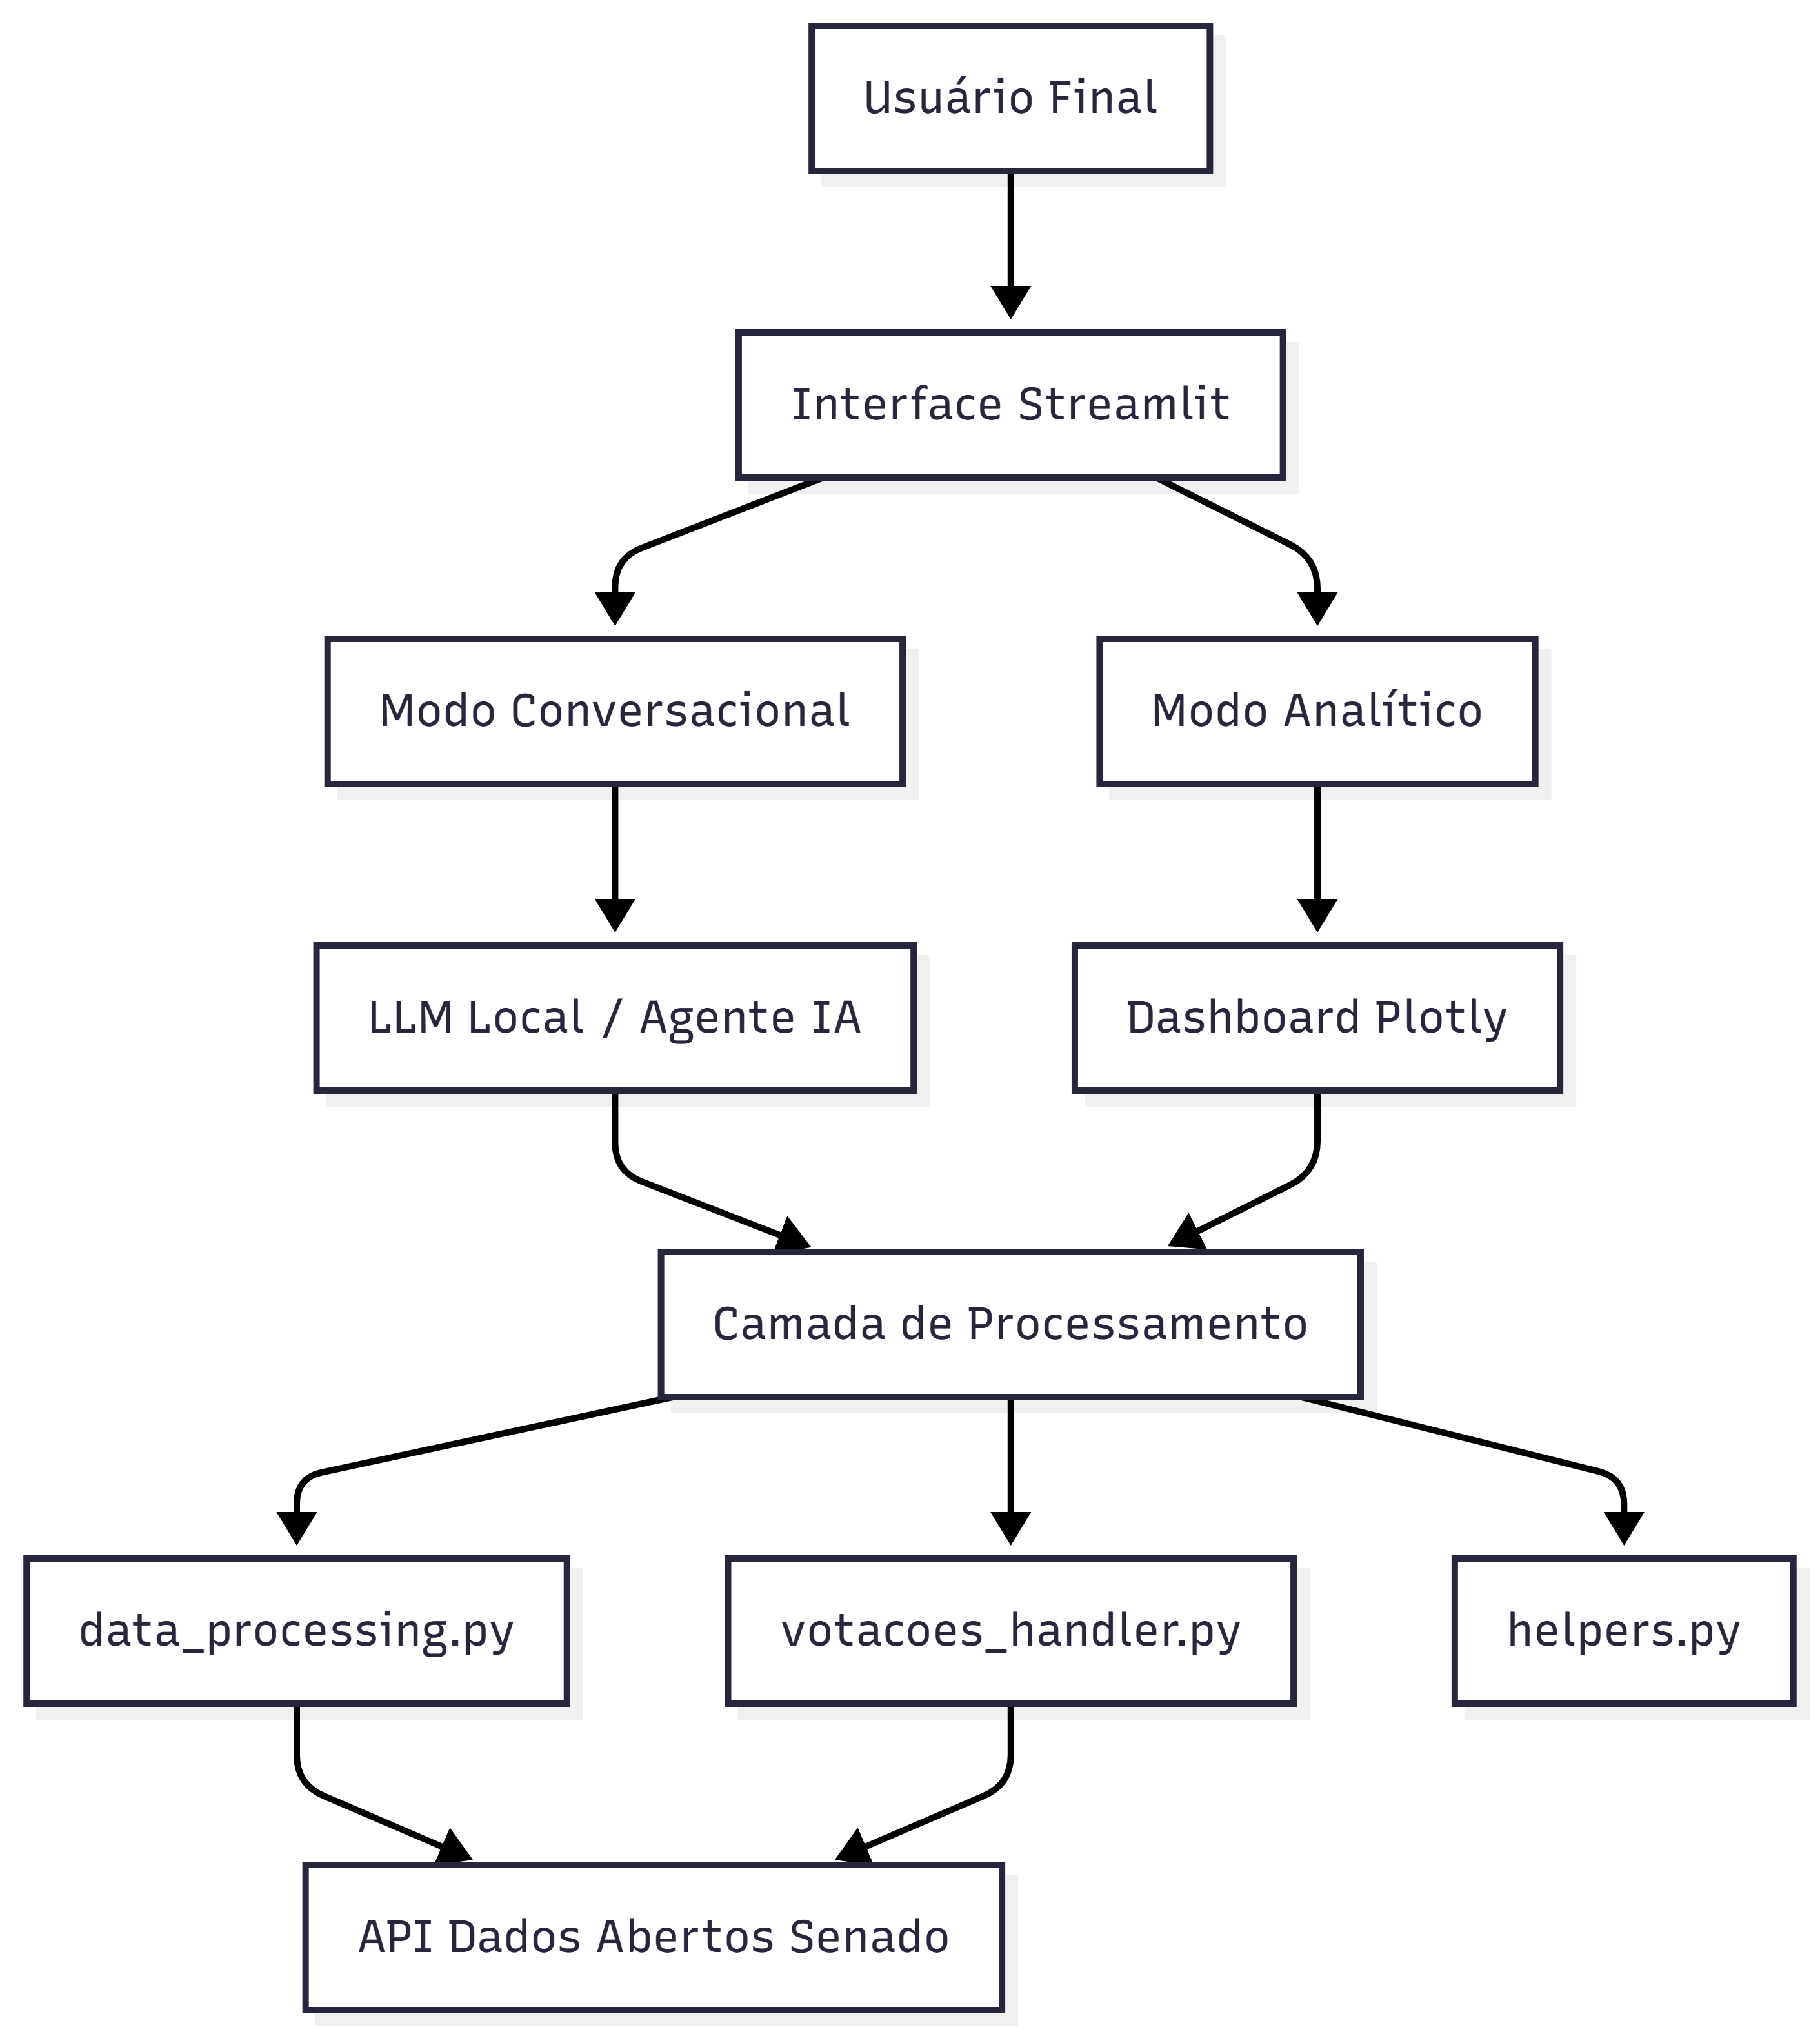
\includegraphics[width=0.9\textwidth]{imagens/arquitetura_aplicacao.png}
\fonte{Produção da autora.}
\end{figure}

Os conceitos discutidos neste capítulo não são independentes entre si: a teoria de dados abertos delimita o corpus e justifica a escolha da API do Senado Federal; os estudos sobre literacia de dados e barreiras cognitivas sustentam a decisão de oferecer duas modalidades de interação (visual e conversacional) em vez de apenas uma; o DSR fundamenta a abordagem metodológica que orienta todo o ciclo de pesquisa; e a discussão sobre RAG e alucinações em LLMs antecipa os desafios concretos que o protocolo de avaliação precisará endereçar. A articulação entre essas dimensões é o que diferencia a proposta de uma simples implementação técnica.